\documentclass[20pt]{article}
\usepackage[a4paper, left=2.0cm, right=2.0cm, top=1.0 cm, bottom=2.5cm]{geometry}
\usepackage[warn]{mathtext}
\usepackage[T2A]{fontenc}
\usepackage[utf8]{inputenc}
\usepackage[russian]{babel}
\usepackage{multirow}
\usepackage{graphicx,wrapfig,lipsum}
\usepackage{xcolor}
\usepackage{pgfplots}
\usepackage{amsmath}
\usepackage[unicode, pdftex]{hyperref}


\begin{document}
    \title{Курсовая работа по вычислительной математике \\ \textbf{№ 9 \\ Стационарная задача теплопроводности в балке }}
        \author{Выполнил Елесин Л. О., Б02-927}
        
    \maketitle

\begin{abstract}
    Получено численное решение стационарной задачи теплопроводоности в балке квадратного сечения при помощи итерационных методов Зейделя, Якоби и верхней релаксации. Получено, что скорость сходимости максимальна при использовании схемы верхней релаксации с параметром $\tau_{opt} = 1.9 $. Также решена нестационрная задача и получена анимация решения.
\end{abstract}
    
\section{Постановка задачи}
    Рассмотрим задачу о нагревании балки квадратного сечения, бесконечной по одной оси координат ($O_{z}$).
    Пусть температура грани AB, BC, CD, DA поддерживается постоянной: 1 на AB, 2 на BC, 3 на CD и 4 на DA (температура приведена в относительных еденицах, $T_{*} = 100^\circ С$). Размер грани AB = BC = CD = AD = 0.1 м. Требуется найти устоявшееся распределение температуры внутри балки.
    \begin{figure}[h!]
        \centering
        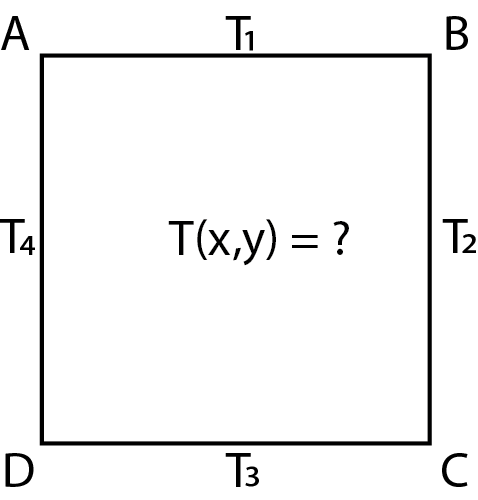
\includegraphics{puzzle.png}
        \caption{Постановка задачи}
        \label{setup}
    \end{figure}
 
\section{Численные методы и граничные условия}
    Стационарное уравнение теплопроводности в 2D имеет вид:
    $$\frac{\partial ^2T(x,y)}{\partial x^2} + \frac{\partial ^2T(x,y)}{\partial y^2} = 0$$
    После дискретезации уравнения, вводя пространственную сетку, используем схему с центральной разностью и получаем :
    $$\frac{T_{i-1,j}-2T_{i,j}+T_{i+1,j}}{\Delta x^2} + \frac{T_{i,j-1}-2T_{i,j}+T_{i,j+1}}{\Delta y^2} = 0{}$$
    Поскольку задача симметрична примем $\Delta x = \Delta y$, и выразим $T_{i,j}$:
    $$T_{i,j} = \frac{T_{i-1,j}+T_{i+1,j}+T_{i,j-1}+T_{i,j+1}}{4}$$
    Будем использоваьть три метода для решения задачи:
     \begin{enumerate}
     \item $\textbf{Метод Якоби.}$ Для вычисления температуры используются только значения из прошлой итерации:
     $$T^{k+1}_{i,j} = \frac{T^{k}_{i-1,j}+T^{k}_{i+1,j}+T^{k}_{i,j-1}+T^{k}_{i,j+1}}{4}$$
     \item $\textbf {Метод Зейделя.}$ Используется как значения из текущей так и из прошлой итерации:
     $$T^{k+1}_{i,j} = \frac{T^{k+1}_{i-1,j}+T^{k}_{i+1,j}+T^{k+1}_{i,j-1}+T^{k}_{i,j+1}}{4}$$
     \item $\textbf {Метод верхней релаксации.}$ К методу Зейделя добавляется коэффициент масштабирования, благодаря которому уменьшается колличество итераций:
     $$T^{k+1}_{i,j} = \frac{T^{k+1}_{i-1,j}+T^{k}_{i+1,j}+T^{k+1}_{i,j-1}+T^{k}_{i,j+1}}{4/\tau} + (1 - \tau)\*T^{k}_{i,j}$$
     \end{enumerate}
    Размер сетки выберем из физических соображений, таких что температуру легко измерять с точностью до сотых на масштабе 1 мм. Так как длина ребра поперечного сечения у нас 10 см, то получится сетка размером 100$\textbf{x}$100. 
    Для критерия остновки будем пользоваться $\textbf{C}$ нормой матрицы распределения темпераутры  $$\frac{\|abs(T^{k-1} - T^{k})\|_{C}}{100 } \leq \epsilon$$ где 100 коэффициент порядка характерной температуры, $\epsilon = 10^{-4}$ выбрана из соображения значения относительной погрешности измерения температуры в реальной жизни.
    

\section{Скорость сходимости и сходимость по сетке}
    Сравним три метода по скорости сходимости на различных сетках. Для этого просто посчитаем количество итераций, после выполнения которых выполняется критерий остановки.
    $$
    \begin{tabular}{|c|r|r|r|r|r|r|r|r|r|}
    \hline
    Length, N_{cells} & 10 & 25 & 50 & 75 & 100 & 125 & 150 & 175 & 200 \\
    \hline
    Jacobi, N_{it} & 47 & 250 & 766 & 1383 & 2013 & 2599 & 3096 & 3470 & 3706 \\
    \hline
    Seidel, N_{it} & 26 & 140 & 448 & 840 & 1274 & 1721 & 2157 & 2565 & 2928 \\
    \hline
    Relax, N_{it} & 18 & 53 & 182 & 357 & 565 & 795 & 1040 & 1294 & 1551 \\
    \hline
    \multicolumn{10}{c}{Таблица 1. Колличество итерраций} \\
    \end{tabular}
    $$
    Теоретические рассчеты дают:
    \begin{enumerate}
     \item Якоби : $I \approx 2\*\frac{N^{2}_{c}}{\pi^2}\*\ln{\epsilon^{-1}}$, $I(100) \approx 9000$
     \item Зейдель: $I \approx \frac{N^{2}_{c}}{\pi^2}\*\ln{\epsilon^{-1}}$, $I(100) \approx 4000$
     \item Релаксация: $I \approx 2\*\frac{N_{c}}{\pi}\*\ln{\epsilon^{-1}}$, $I(100) \approx 300$
     \end{enumerate}
     Что по порядку велечины совпадает с численными расчетами, и отражает тот факт, что метод Якоби самый медленный, а верхней релоксации самый быстрый.
    \begin{figure}[h!]
        \centering
        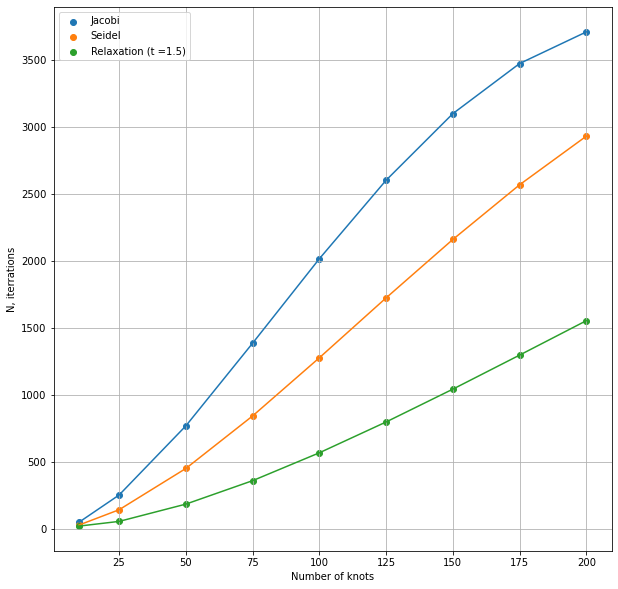
\includegraphics[width=80mm]{shod.png}
        \caption{Скорость сходимости в зависимости от колличества узлов}
        \label{setup}
    \end{figure}
    \newpage
    Убедимся, что методы сходятся по сетке, для этого будем вычислять среднюю температуру на разных линиях, измельчая сетку. Посчитаем средние значения на высоте 2, 4, 6 и 8 см, и убедимся, что при измельчении сетки среднее значение выходит на плато.
    \begin{figure}[h!]
        \centering
        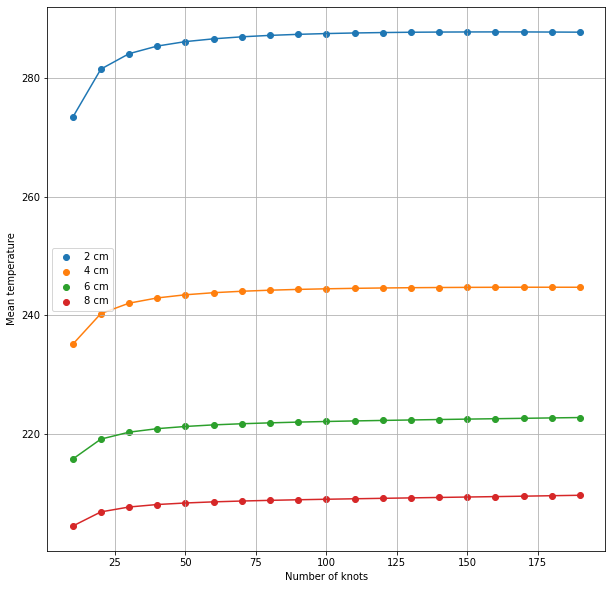
\includegraphics[width=55mm]{mean_hor.png}
        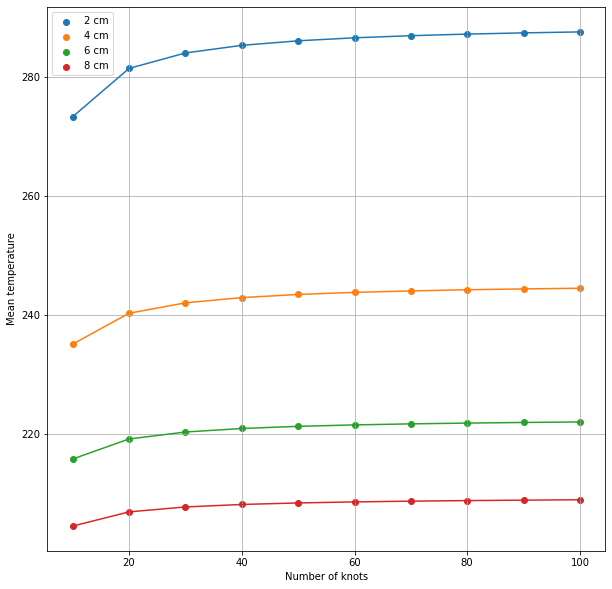
\includegraphics[width=55mm]{mean_hor_2.png}
        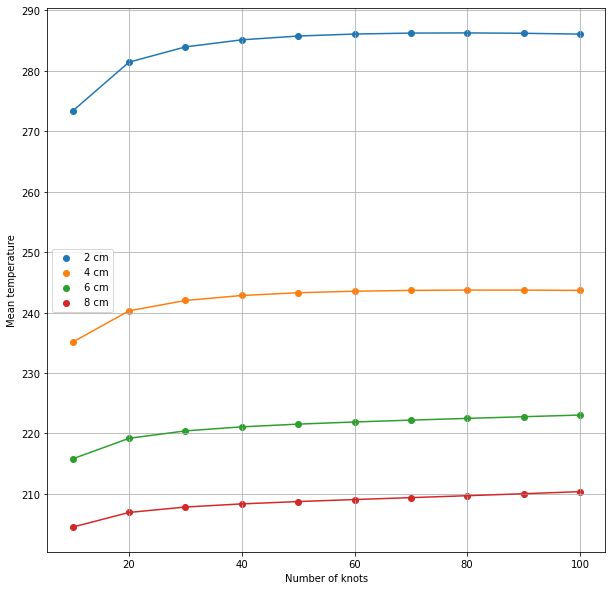
\includegraphics[width=55mm]{mean_hor_3.png}
        \caption{Сходимость по сетке (Релаксация, Якоби, Зейдель)}
        \label{setup}
    \end{figure}

\section{Зависимость скорости сходимости метода верхней релаксации от параметра $\tau$}
    На сетке 100x100 исследуем скорость сходимости метода верхней релаксации в зависисмости от параметра $\tau$. Видно, что скорость сходимости максимальна при $\tau \approx 1.9$.
    \begin{figure}[h!]
        \centering
        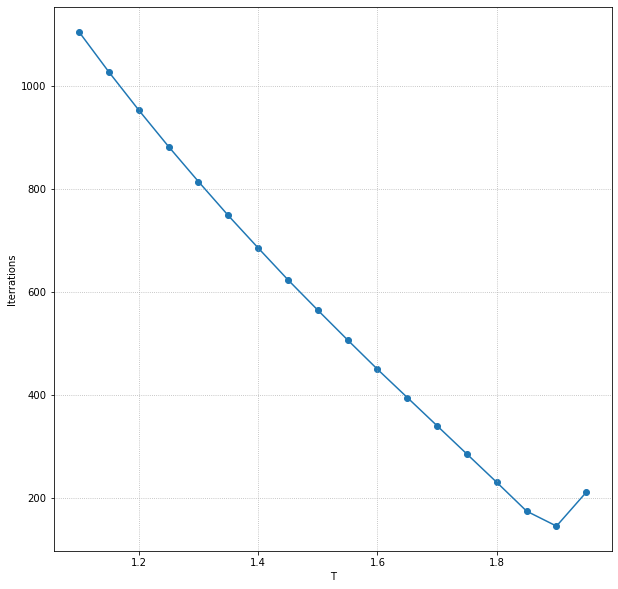
\includegraphics[width=80mm]{tau.png}
        \caption{Скорость сходимости в зависисмости от параметра $\tau$}
        \label{setup}
    \end{figure}
    
 
\section{Результаты численного моделирования}
    Приведем основные результаты полученные численными методами, на основной сетке (100x100), а именно графики зависисмости T(x,y), графики T(x) при фиксированном y и T(y) при фиксированном x. 
    \newpage
    \begin{figure}[h!]
        \centering
        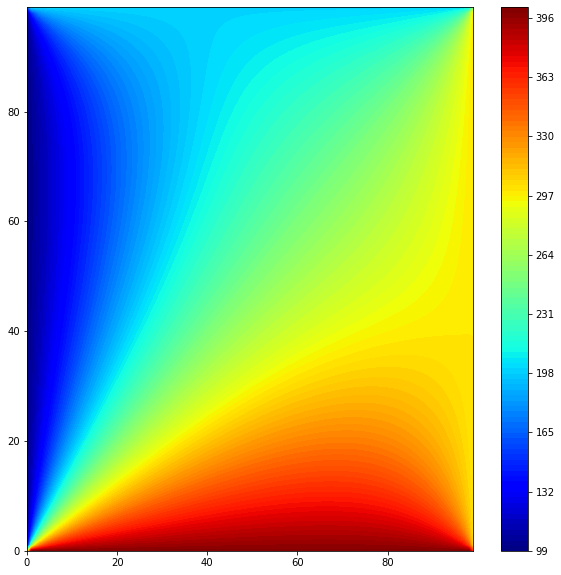
\includegraphics[width=55mm]{jacobi.png}
        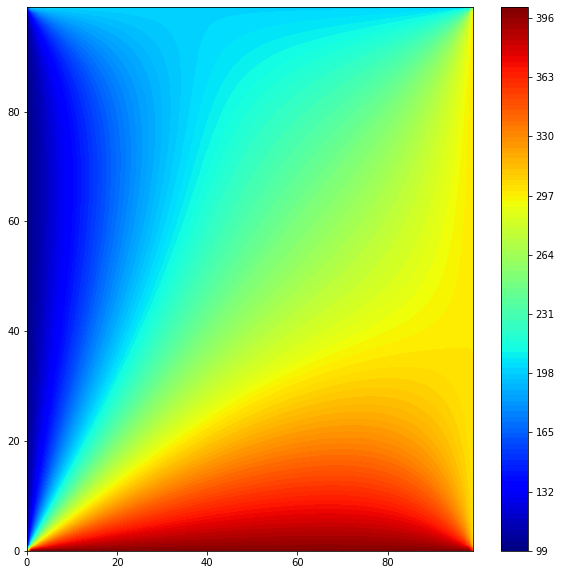
\includegraphics[width=55mm]{seidel.png}
        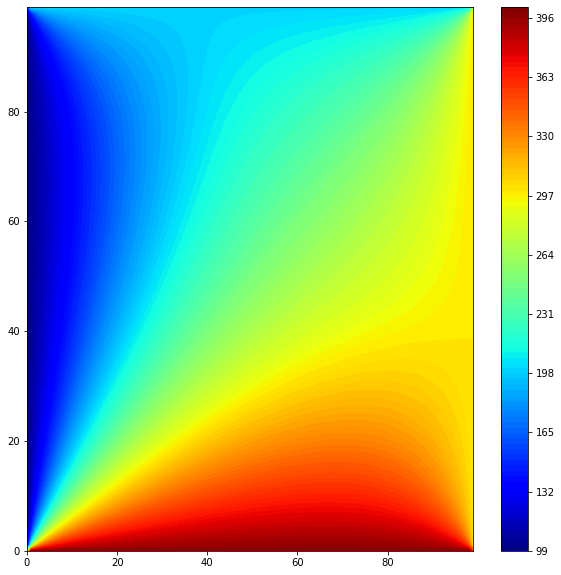
\includegraphics[width=55mm]{relax.png}
        \caption{Изолинии (Якоби, Зейдель, Релаксация)}
        \label{setup}
    \end{figure}
    \begin{figure}[h!]
        \centering
        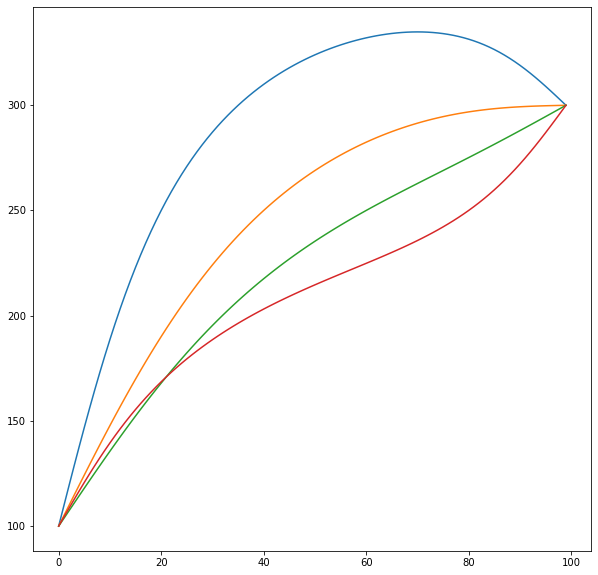
\includegraphics[width=55mm]{x_seidel.png}
        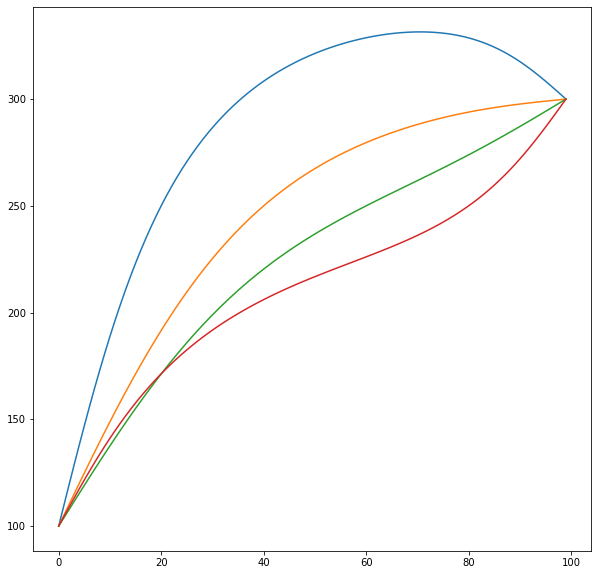
\includegraphics[width=55mm]{x_jacobi.png}
        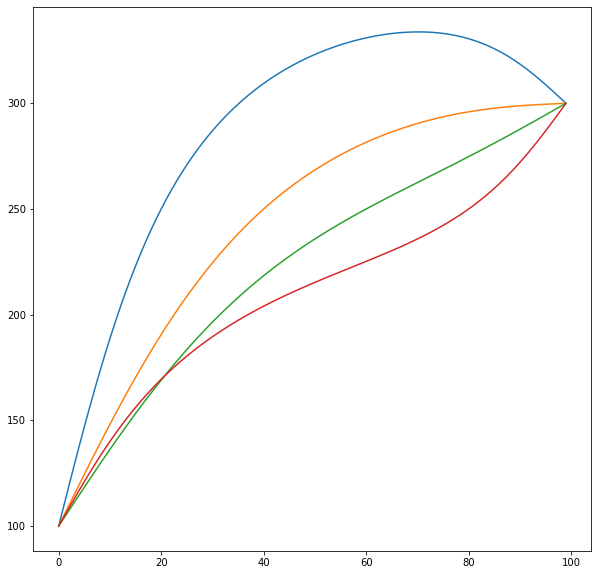
\includegraphics[width=55mm]{x_relax.png}
        \caption{Зависимость температуры при фиксированном X (Якоби, Зейдель, Релаксация)}
        \label{setup}
    \end{figure}
    \begin{figure}[h!]
        \centering
        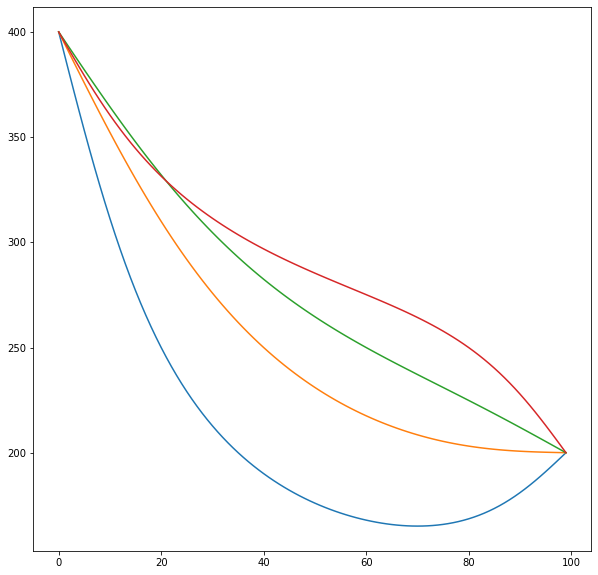
\includegraphics[width=55mm]{y_jacobi.png}
        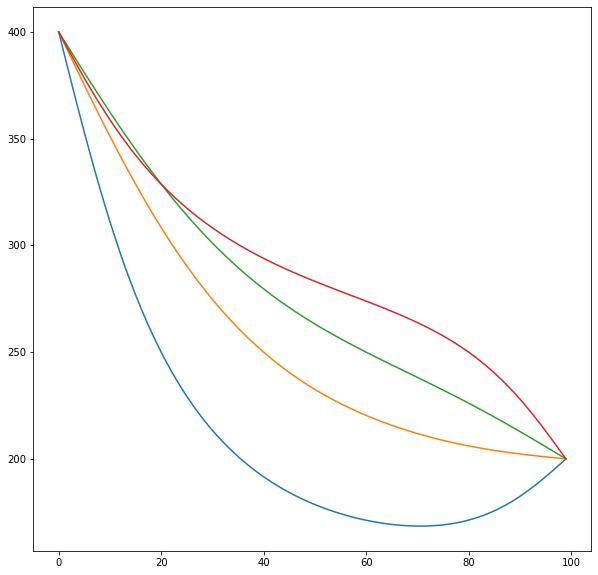
\includegraphics[width=55mm]{y_seidel.png}
        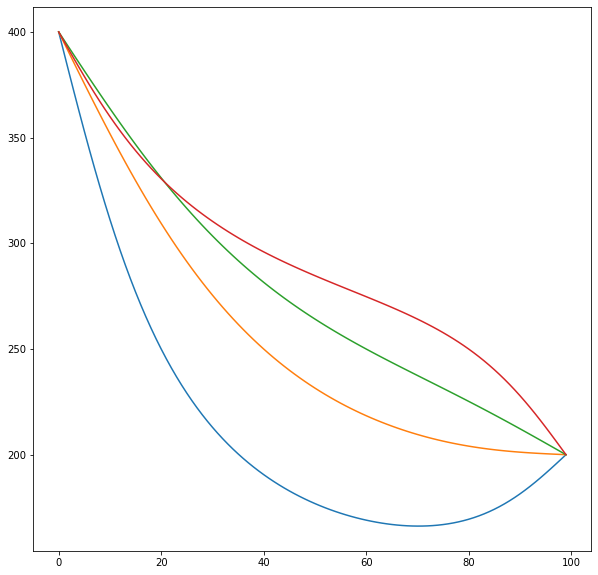
\includegraphics[width=55mm]{y_relax.png}
        \caption{Зависимость температуры при фиксированном Y (Якоби, Зейдель, Релаксация)}
        \label{setup}
    \end{figure}

\section{Вывод}
Получено численное решение стационарной задачи теплопроводоности в балке квадратного сечения при помощи итеррационных методов Зейделя, Якоби и верхней релаксации. Методы показали аналогичные результаты, но самым быстрым по сходимости и по времени работы оказался метод верхней релаксации, также по порядку скорость сходимости совпала с теорией. Получено, что скорость сходимости в схеме верхней релаксации максимальна при использовании параметра $\tau_{opt} = 1.9 $  
\newpage
\section{Приложение}
\subsection{Решение нестационарной задачи}
Нестационарная задача теплопроводности имеет вид:
$$\frac{\partial ^2T(x,y,t)}{\partial x^2} + \frac{\partial ^2T(x,y,t)}{\partial y^2} =\alpha\* \frac{\partial T(x,y,t)}{\partial t}$$
Где $\alpha$ - коэффициент температуропроводности. Например для некоторых композитов углерода $\alpha \approx 0.00025\ m^{2}/s$.
Дискретезируя уравнение и выражая температуру получим (используя явный метод):
$$T^{k+1}_{i,j} = T^{k}_{i,j} + \alpha\*\frac{\Delta\*t}{\Delta\*h^{2}}\*( T^{k}_{i-1,j}+T^{k}_{i+1,j}+T^{k}_{i,j-1}+T^{k}_{i,j+1}-4\*T^{k}_{i,j})$$
За временную единицу выберем $\Delta\*t = 1\ $мс, за пространственную $\Delta\*x = \Delta\*y = \Delta\*h= 0.001\ $м . Решая численно получим \href{https://github.com/LeoYe-st/Vychmat_project}{GIF} файл (evolution main), где отображается изменение температуры в образце в зависимости от времени. Также имеются анимации с другими начальными распределениями температуры.
\subsection{Результаты численного моделирования}
Приведена финальная картинка распределения температуры решения стационарного уравнения для метода верхней релаксации. Для метода Зейделя и верхней релаксации получены \href{https://github.com/LeoYe-st/Vychmat_project}{GIF}, отражающие изменение решения в зависимости от итерации.
\begin{figure}[h!]
        \centering
        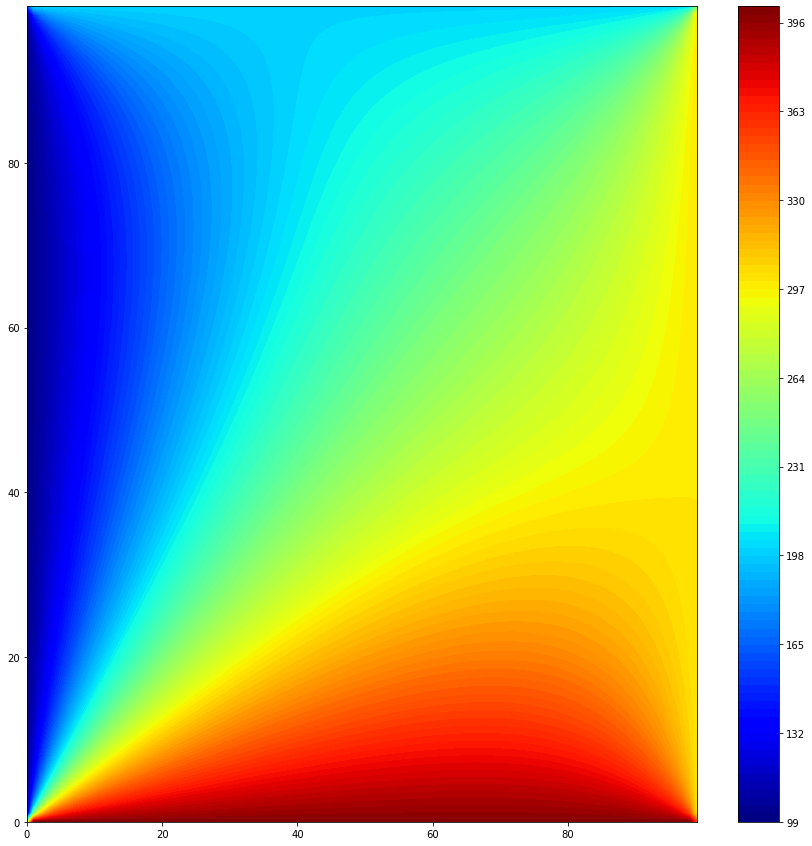
\includegraphics[width=132mm]{final.png}
        \caption{Распределение температуры (Релаксация)}
        \label{setup}
    \end{figure}
\subsection{Ссылка на код и на саму работу}
\url{https://github.com/LeoYe-st/Vychmat_project}
\end{document}
